% VUT FIT MITAI
% MSZ 2021/2022
% Author: Vladimir Dusek
% Login: xdusek27

%%%%%%%%%%%%%%%%%%%%%%%%%%%%%%%%%%%%%%%%%%%%%%%%%%%%%%%%%%%%%%%%%%%%%%%%%%%%%%%%

% Path to figures
\graphicspath{{msp/nahodna_promenna/figures}}

%%%%%%%%%%%%%%%%%%%%%%%%%%%%%%%%%%%%%%%%%%%%%%%%%%%%%%%%%%%%%%%%%%%%%%%%%%%%%%%%

\chapter{MSP~--~Náhodná proměnná, typy náhodné proměnná, funkční a číselné charakteristiky, významná rozdělení pravděpodobnosti.}

%%%%%%%%%%%%%%%%%%%%%%%%%%%%%%%%%%%%%%%%%%%%%%%%%%%%%%%%%%%%%%%%%%%%%%%%%%%%%%%%

\section{Zdroje}

\begin{compactitem}
    \item \path{MSP_pred_01_Opakovani_Pravd-NP-NV.pdf}
    \item \path{MSP_pred_02_Opakovani_Statistika_Regrese.pdf}
\end{compactitem}

%%%%%%%%%%%%%%%%%%%%%%%%%%%%%%%%%%%%%%%%%%%%%%%%%%%%%%%%%%%%%%%%%%%%%%%%%%%%%%%%

\section{Náhodná proměnná}

\begin{compactitem}
    \item Náhodná proměnná (také náhodná veličina) je funkce, reprezentuje nějaký náhodný proces. Přiřazuje každému elementárnímu náhodnému jevu nějakou (zpravidla číselnou) hodnotu. \begin{compactitem}

        % \item Náhodnou veličinu lze jednoduše charakterizovat jako veličinu, jejíž hodnoty nelze před provedením pozorování jednoznačně určit, ale závisí na náhodě.

        \item Příklad náhodné proměnné reprezentující náhodný proces hod mincí:
        $$ X = \left\{
            \begin{array}{ll}
                1 & \text{pokud padne \uv{hlava}} \\
                0 & \text{pokud padne \uv{orel}}
            \end{array}
            \right.$$

        Zkoumání pravděpodobnosti:
        $$ P(X = 1) = \ldots$$

    \end{compactitem}

    \item \textbf{Formálně} -- Nechť $\Omega$ je základní prostor a $(\Sigma, \Omega)$ je jevové pole. Pak zobrazení $X : \Omega \rightarrow \mathbb{R}$ se nazývá náhodná proměnná, pokud je měřitelné, tj.
    $$\forall x \in \mathbb{R} : \{ \omega \in \Omega ~|~ X(\omega) < x \} \in \Sigma$$

    \item Realizaci náhodné veličiny, tj. $X(\omega),~ \omega \in \Omega$ označíme $x$, pak \begin{compactitem}
        \item množinu $\{ \omega \in \Omega ~|~ X(\omega) < x \}$ zapisujeme jako $\{ X < x \}$,

        \item množinu $\{ \omega \in \Omega ~|~ X(\omega) = x \}$ zapisujeme jako $\{ X = x \}$.
    \end{compactitem}

    % \item Mějme hodnoty $x_1$ a $x_2$, příklad vyjádření pravděpodobnosti vzhledem k náhodné proměnné $X$:
    % $$ P(x_1 < X < x_2) $$

    % \item Pro obor hodnot náhodné proměnné $X$ $$ Z = \{ x \in \mathbb{R} ~|~ \exists \omega \in \Omega : x = X(\omega) \} $$
\end{compactitem}

\subsection{Distribuční funkce}

\begin{compactitem}
    \item Hodnota $P(\{ \omega \in \Omega ~|~ X(\omega) < x \})$ se nazývá distribuční funkce náhodné veličiny $X$ a značí se $F(x)$.

    \item Zkráceně zapisujeme jako $F(x) = P(X < x) ~,~ \forall x \in \mathbb{R}$.

    \item Distribuční funkce udává, že hodnota náhodné proměnné je menší než zadaná hodnota.

    \item Vlastnosti: \begin{compactitem}

        \item DF je zprava spojitá,
        $$ \lim_{x \rightarrow \alpha^{+}} F(x) = F(\alpha) $$

        \item DF je neklesající,
        $$ \alpha < \beta \Rightarrow F(\alpha) \leq F(\beta) $$

        \item asymptotické vlastnosti:
        $$ \lim_{x \rightarrow - \infty} F(x) = 0 $$
        $$ \lim_{x \rightarrow + \infty} F(x) = 1 $$
    \end{compactitem}

\end{compactitem}

%%%%%%%%%%%%%%%%%%%%%%%%%%%%%%%%%%%%%%%%%%%%%%%%%%%%%%%%%%%%%%%%%%%%%%%%%%%%%%%%

\section{Diskrétní náhodná proměnná}

\begin{compactitem}
    \item Náhodná proměnná se nazývá \textbf{diskrétní}, pokud základní soubor $Z \subset \mathbb{R}$ je konečná nebo nejvýše spočetně nekonečná množina.

    \item \textbf{Pravděpodobnostní funkce} \begin{compactitem}
        \item Udává pravděpodobnost, že diskrétní náhodná veličina se přesně rovná nějaké hodnotě.

        \item Funkci $p(x) = P(X = x) ~,~ x \in \mathbb{R}$ nazýváme pravděpodobností funkcí diskrétní náhodné veličiny $X$.

        \item Platí:
        $$ \sum_{i=1}^n p(x_i) = 1 $$
        $$ \forall x \in Z ~:~ 0 \leq p(x) \leq 1$$
    \end{compactitem}

    \begin{figure}[H]
        \centering
        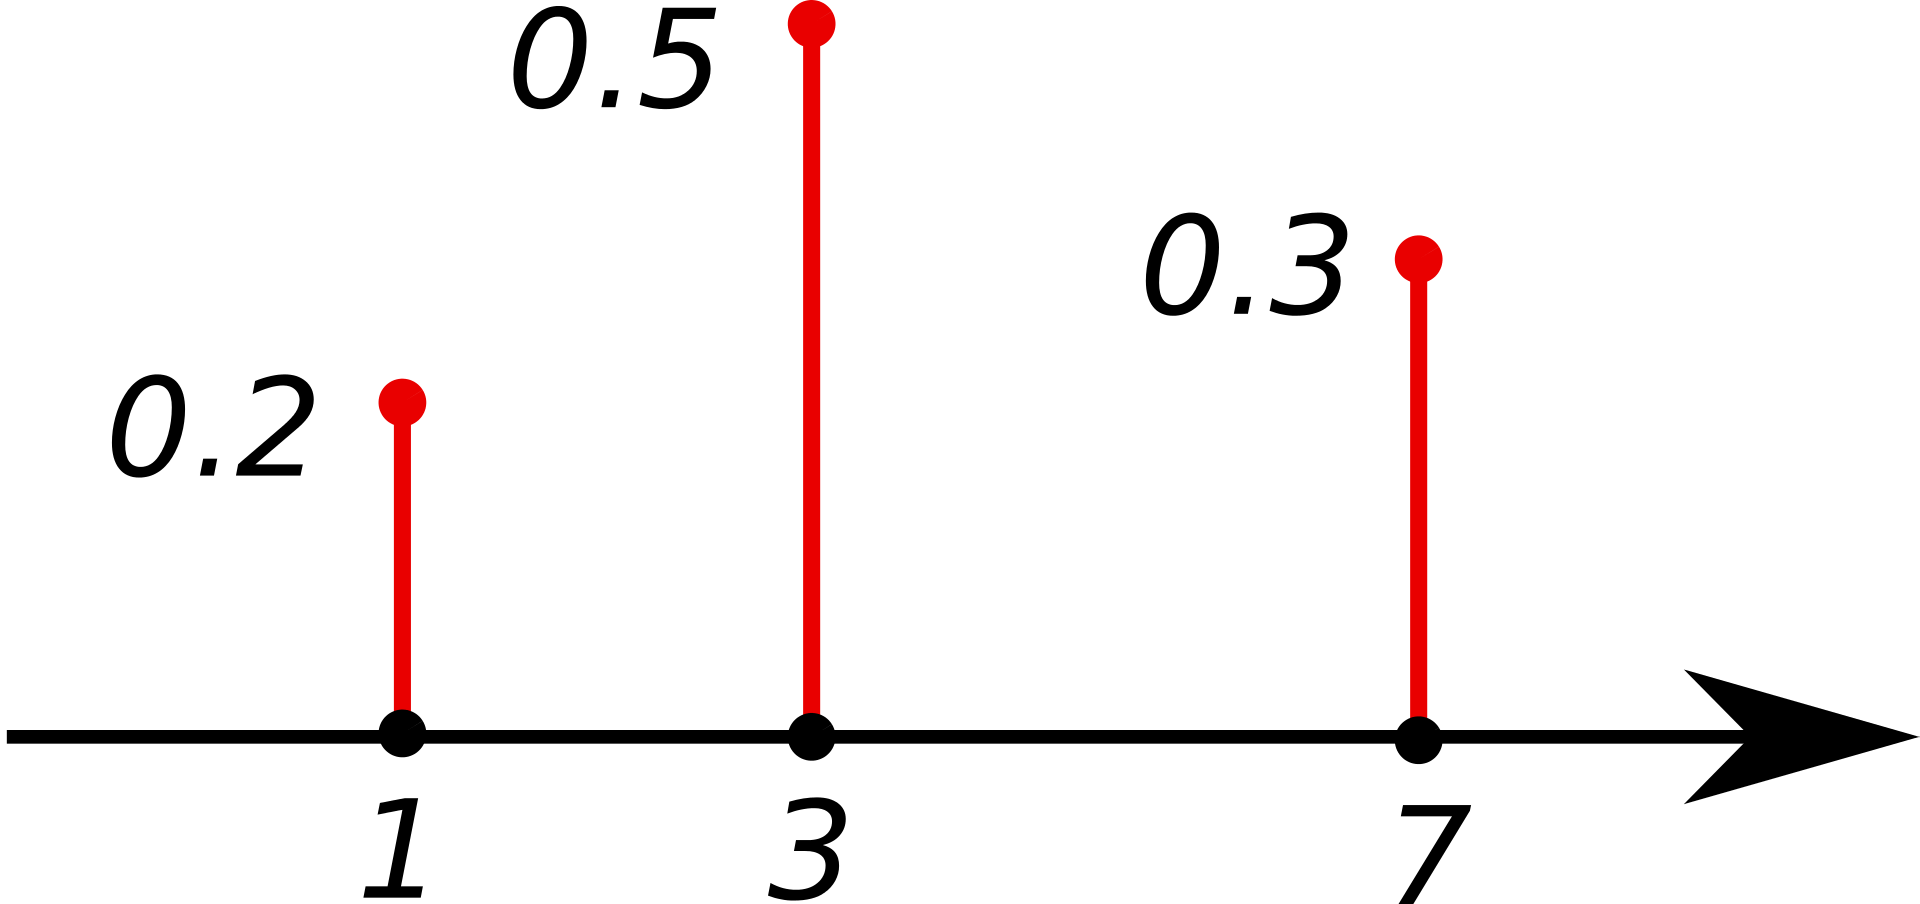
\includegraphics[width=0.5\linewidth]{dnp_pravdepodobnostni_funkce.png}
        \caption{Příklad pravděpodobnostní funkce pro DNP.}
    \end{figure}

    \item \textbf{Distribuční funkce} \begin{compactitem}
        \item Distribuční funkce má tvar:
        $$ F(x) = \sum_{t < x} p(t) ~,~ \forall x \in (-\infty, +\infty)$$

        \item Platí: \todo{Todo: overit}
        $$ p(x) = \lim_{t \rightarrow x+} F(t) - F(x) $$
    \end{compactitem}

    \begin{figure}[H]
        \centering
        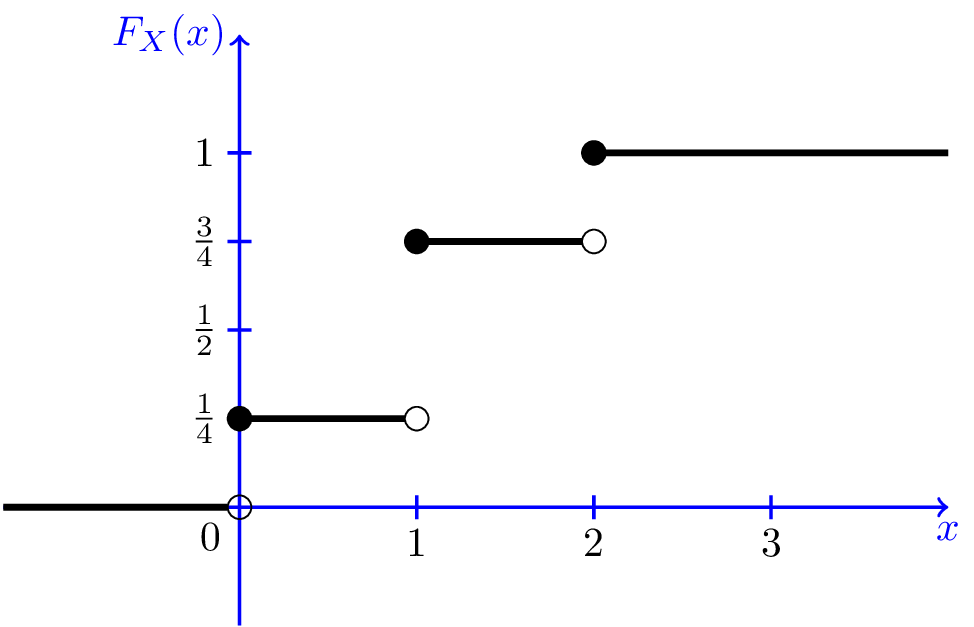
\includegraphics[width=0.75\linewidth]{dnp_distribucni_funkce.png}
        \caption{Příklad distribuční funkce pro DNP.}
    \end{figure}

    \item \textbf{Příklad} -- náhodná proměnná reprezentující součet hodnot po 5 hodech šestistrannou kostkou.
    $$ X = \text{suma 5 hodů šestistrannou kostkou} $$ \begin{compactitem}
        \item Zkoumání pravděpodobnosti, že součet bude větší než 15:
            $$ P(X > 15) = \ldots$$
    \end{compactitem}

\end{compactitem}

%%%%%%%%%%%%%%%%%%%%%%%%%%%%%%%%%%%%%%%%%%%%%%%%%%%%%%%%%%%%%%%%%%%%%%%%%%%%%%%%

\section{Spojitá náhodná proměnná}

\begin{compactitem}
    \item Náhodná proměnná se nazývá \textbf{spojitá}, pokud základní soubor $Z \subseteq \mathbb{R}$ je nekonečná nespočetná množina a existuje nezáporná, po částech spojitá funkce $f(x)$, taková, že
    $$ F(x) = \int_{- \infty}^{x} f(t) ~ dt ~,~ x \in \mathbb{R} $$

    \item Pravděpodobnost konkrétní hodnoty je $0$, formálně:
    $$ \forall c \in \mathbb{R} : P(X=c) = 0$$

    \item \textbf{Funkce fustoty pravděpodobnosti} \begin{compactitem}
        \item Funkci $f : \mathbb{R} \rightarrow \mathbb{R}^{+}$ nazýváme funkci hustoty pravděpodobnosti náhodné veličiny $X$.

        \item Platí:
        $$  $$
        $$ \int_{- \infty}^{+ \infty} f(x) ~ dx = 1$$
    \end{compactitem}

    \begin{figure}[H]
        \centering
        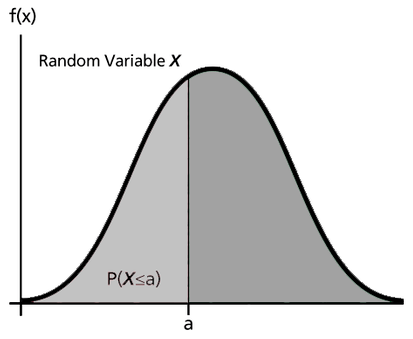
\includegraphics[width=0.5\linewidth]{snp_probability_density_function.png}
        \caption{Příklad funkce hustoty pravděpodobnosti pro SNP.}
    \end{figure}

    \item \textbf{Distribuční funkce} \begin{compactitem}
        \item Má tvar:
        $$ F(x) = \int_{- \infty}^{x} f(t) ~ dt ~,~ x \in \mathbb{R} $$

        \item Platí, nechť $a, b \in \mathbb{R}$:
        $$ P(x < a) = P(x \leq a) = F(a) $$
        $$ P(a < x < b) = P(a \leq x \leq b) = \int_a^b f(x) ~ dx = F(b) - F(a) $$
    \end{compactitem}

    \begin{figure}[H]
        \centering
        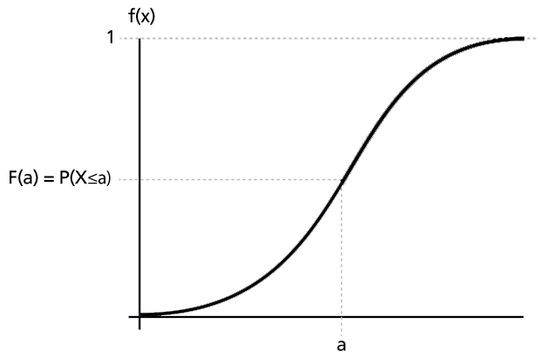
\includegraphics[width=0.5\linewidth]{snp_distribution_function.png}
        \caption{Příklad distribuční funkce pro SNP.}
    \end{figure}

    \item \textbf{Příklad} -- náhodná proměnná reprezentující čas běhu závodníka v běhu na 100\,m.
    $$ X = \text{čas běhu na 100\,m} $$ \begin{compactitem}
        \item Zkoumání pravděpodobnosti, že zaběhne pod 10:
            $$ P(X < 10) = \ldots$$
    \end{compactitem}

\end{compactitem}

%%%%%%%%%%%%%%%%%%%%%%%%%%%%%%%%%%%%%%%%%%%%%%%%%%%%%%%%%%%%%%%%%%%%%%%%%%%%%%%%

\section{Číselné charakteristiky náhodné proměnné}

\begin{compactitem}
    \item Dělíme na: \begin{compactitem}
        \item charakteristiky polohy -- střední hodnota, medián, modus;
        \item charakteristiky variability -- rozptyl, směrodatná odchylka.
    \end{compactitem}
\end{compactitem}

\begin{compactitem}

    \item \textbf{Kvantil} -- Kvantil je charakteristika, kterou stanovená část $p$ (uváděná jako číslo z intervalu $\langle 0, 1\rangle$) hodnot nepřesahuje. Je také možné říct, že kvantily jsou hodnoty, které dělí soubor seřazených (například naměřených) hodnot na několik zhruba stejně velkých částí. (Příklad: výrok, že 90\,\% účastníků závodu mělo čas pod 2 hodiny, vlastně konstatuje, že 90. percentil dosažených časů je 2 hodiny.)

    \item \textbf{Medián} -- Nechť $p \in \langle 0, 1\rangle$ je kvantil náhodné proměnné. Pokud $p = 0,5$, tak se $p$ kvantil nazývá medián a značí se $\tilde{x}$.

    \item \textbf{Modus} -- Modus náhodné veličiny $X$ je reálné číslo $\hat{x}$, které je maximem pravděpodobnostní funkce, resp. funkce hustoty pravděpodobnosti.

    \item \textbf{Střední hodnota} -- Střední hodnota (také očekávaná hodnota) diskrétní náhodné proměnné je pravděpodobnostně vážený průměr všech jejích možných hodnot, pro spojitou náhodnou proměnnou je součet nahrazen integrálem proměnné vzhledem k její hustotě pravděpodobnosti. \begin{compactitem}
        \item Značí se:
        $$ E(X) ~,~ \mu(X) $$

        \item Pro DNP:
        $$ E(X) = \sum_{i = 1}^n x_i \cdot p(x_i) $$

        \item Pro SNP:
        $$ E(X) = \int_{- \infty}^{+ \infty} x \cdot f(x) ~ dx $$
    \end{compactitem}

    \item \textbf{Rozptyl} -- Rozptyl (také střední kvadratická odchylka, variance) je druhý centrální moment náhodné veličiny. Jedná se o charakteristiku variability rozdělení pravděpodobnosti náhodné veličiny, která vyjadřuje variabilitu rozdělení souboru náhodných hodnot kolem její střední hodnoty. \begin{compactitem}
        \item Značí se:
        $$ D(X) ~,~ S^2(X) ~,~ \sigma^2(X) $$

        \item Pro DNP:
        $$ D(X) = \sum_{i=1}^n {\left(x_i - E(X)\right)}^2 \cdot p_i $$

        \item Pro SNP:
        $$ D(X) = \int_{-\infty}^\infty {\left( x - E(X) \right)}^2 \cdot p(x) ~ dx = \int_{-\infty}^\infty x^2 \cdot p(x) ~ dx - E(X)^2 $$
    \end{compactitem}

    \item \textbf{Směrodatná odchylka} -- Je odmocnina rozptylu náhodné veličiny. \begin{compactitem}
        \item Značí se:
        $$ S(X) ~,~ \sigma(X) $$

        \item Pro DNP, SNP:
        $$ \sigma(X) = \sqrt{D(X)} $$
    \end{compactitem}

    \item \textbf{Šikmost, špičatost, čebyšova nerovnost} \begin{compactitem}
        \item \textit{Nepředpokládám, že by se zkoušelo.}
    \end{compactitem}

    \item \textbf{Kovariance, korelace} -- Charakteristiky pro popis vzájemného vztahu dvou veličin. \begin{compactitem}
        \item \textit{Nepředpokládám, že by se zkoušelo.}
    \end{compactitem}
\end{compactitem}

%%%%%%%%%%%%%%%%%%%%%%%%%%%%%%%%%%%%%%%%%%%%%%%%%%%%%%%%%%%%%%%%%%%%%%%%%%%%%%%%

\section{Vybraná rozdělení diskrétní náhodné proměnné}

\subsection{Alternativní (Bernoulliho) rozdělení}

\todo{todo}

\subsection{Klasické rozdělení}

\todo{todo}

\subsection{Binomické rozdělení}

\todo{todo}

\subsection{Poissonovo rozdělení}

\todo{todo}

%%%%%%%%%%%%%%%%%%%%%%%%%%%%%%%%%%%%%%%%%%%%%%%%%%%%%%%%%%%%%%%%%%%%%%%%%%%%%%%%

\section{Vybraná rozdělení spojité náhodné proměnné}

\subsection{Rovnoměrné rozdělení}

\todo{todo}

\subsection{Exponenciální rozdělení}

\todo{todo}

\subsection{Normální (Gaussovo) rozdělení}

\todo{todo}
